\chapter{Software}

\section{Communication Core}
Paul -done

\section{CarControl Core}
The \textbf{CarControl Core} is responsible for processing all the data that the communications core receives from other components, and calculating the correct reactions (Motor Controller signals) to that data. 

\subsection{Location}
The CarControl Core software project resides in $software/Car2X\_carControl$; the $.sopcinfo$ file used to generate the board support package here: \\$hardware/nios\_system.sopcinfo$. The software runs on Core 1 of the system.

\subsection{Program flow}
The control core cyclically accesses the current $CarState$ from the shared memory and performs all calculations. The main loop can be broken down into four parts.

\begin{enumerate}
\item Get current $CarState$ from the shared memory (blocking).
\item Check the operating mode, $state.reqOpMode$. If a new one has been requested, the transition is performed and set in $state.currOpMode$.
\item Get the requested velocities $state.reqVel$ and transform them into goal velocities for each wheel. These are then written into $state.MotorECU\_State$.
\item Write the changed $CarState$ object back into the shared memory and release the mutex.
\end{enumerate}

\subsection{Operating modes}
A state machine is used to restrict or alter the car's behaviour, based on the current \textbf{Operating mode} of the car. Broadly speaking, an Operating Mode places restrictions on what actors can control the car at any given time, and the velocity at which the car may move. Some Operating Modes are used internally, while others can be requested by the user.

\begin{description} 
\item[PreOperational] Initial mode, used internally during the startup phase. The velocity is restricted to $0$ on all motors.
\item[Idle] This operating mode is automatically transitioned to upon successful communication with all four Motor Control ECUs. Velocity is restricted to $0$ on all motors.
\item[AutomaticDrive] This mode is to be used when the car drives autonomously. The car may only be controlled from the IP address that is registered as the autonomous driving component (the image processing component in our case). The velocity is restricted to $200mm/s$.
\item[ManualDrive] A $RemoteControlMessage$ C2X message will transition the car into this mode. Subsequently, the car may only be controlled from the IP address that sent the aforementioned message. The velocity is restricted to $400mm/s$.
\item[EmergencyStop] Triggered by an $EmergencyBrakeMessage$, this operation mode will immediately set all motor velocities to $0$, effectively executing an emergency stop. To exit this operating mode, either a $RemoteControlMessage$ must be sent.
\end{description}

\subsection{Motor velocity calculation}
The motor velocity calculations are relatively straightforward. Each operating mode has a maximum velocity that may be requested. Any velocities above this limit are scaled down to the limit. Equations \eqref{carcontrol:avel_calc} \eqref{carcontrol:vel_calc} show how the scaling is performed.

\begin{equation}
\label{carcontrol:avel_calc}
v_{limit} = \frac{1}{4} \sum_{i=1}^{4} v_i 
\end{equation}

\begin{equation}
\label{carcontrol:vel_calc}
v_{i} = 
\begin{cases}
r_{i} & \mbox{if } r_{avg} \leq v_{limit} \\
v_{limit}/r_{avg} * r_{i} & \mbox{if } r_{avg} > v_{limit} \\
\end{cases}
\end{equation}

Since the velocities are transmitted as signed 16bit integer values, integer arithmetic is used to calculate the goal velocity, at a precision of $0.01mm/s$.

\section{Shared memory}
The \textbf{Shared Memory Module} is responsible for ensuring the safe exchange of data between the Communication and the CarControl cores. On the hardware level, the \textbf{Shared Memory} and \textbf{Hardware Mutex} building blocks provide the necessary foundations that the \textbf{$MemController$} class leverages. Figure \ref{sharedmem:pic_overview} shows a conceptual representation of the Shared Memory Module and its components in action.

\begin{figure}[h]\label{sharedmem:pic_overview}
  \caption{The shared memory setup. The Hardware components are shaded in blue, the components of the Shared Memory Software Module are shaded orange.}
  \centering
    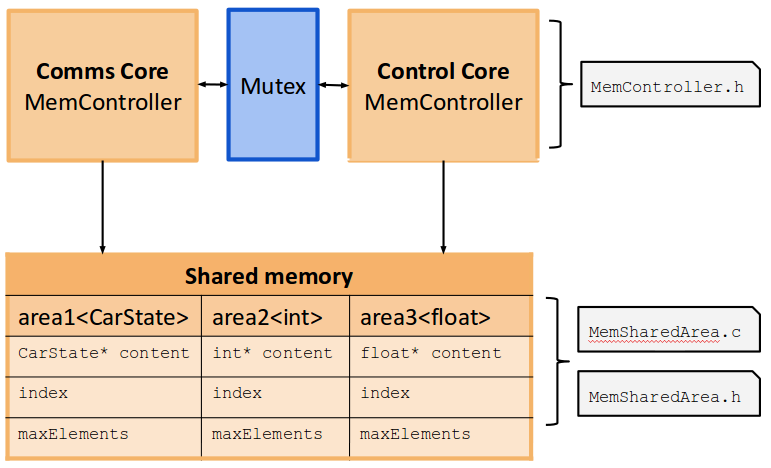
\includegraphics[width=1.0\textwidth]{figures/shared_memory.png}
\end{figure}

\subsection{Location}
The $MemController$ Class resides in $software/shared\_files/MemController.h$. The $MemSharedArea$ is declared in $software/shared\_files/MemSharedArea.h$, with the variable allocation occuring in $MemSharedArea.cpp$.

\subsection{Shared Memory Areas}
The \textbf{$MemSharedArea$} struct (see \ref{sharedmem:code_memsharedarea}) provides a container for managing data in the shared memory. The main goal of the shared memory is to facilitate data exchange between multiple threads/cores.

\begin{lstlisting}[language=C++, label=sharedmem:code_memsharedarea, caption={$MemSharedArea$ structure, the container for shared data. Code found at: $software/ shared\_files/ MemSharedArea.h$}] 
template<typename T>
struct MemSharedArea {
	alt_u32 maxNumElements_u32;
	T * content_a;
	alt_u32 index_u32;
	enum Bufferflags flags_u32;
};
\end{lstlisting}

All containers are declared in $MemSharedArea.c$. Here, the containers are defined and initialised to their default values. In the following snipped, Altera directives are used to instruct the linker to place the variable $AreaCarStateBuffer$ into the hardware memory component titled $.shared\_memory$:
\begin{lstlisting}
CarState AreaCarStateBuffer[BUFFERSIZE_CARSTATE] __attribute__ ((section (".shared_memory")));
\end{lstlisting}
 Note that it is necessary to define both the $MemSharedArea$ container, and the array where the actual content will be stored.

Since the $MemSharedArea$ structure accepts a template argument, any data structure may be stored within the $MemSharedArea$ containers, as long as it can be serialised and there is enough space in memory.

\subsection{Memory controller}
The MemController class provides an interface to access these areas in a safe and ordered fashion. The shared memory area array member is treated as a ring buffer, to allow for a historical retrieval of a certain information stream. 

The primary constructor of a MemController has the following signature:
\begin{lstlisting}
MemController<T>(MemSharedArea<T> * area_p);
\end{lstlisting} 
This creates a MemController object that provides access to the shared memory area $area\_p$. One memory controller is always responsible for just one memory area. Note that the template argument for both the $MemController$ and the $MemSharedArea$ parameter must be the same. 

Currently, there is only one mutex available at the hardware level, so simultaneous access to different shared memory containers is impossible, though it would be safe. A shortened version of the API is shown in snipped \ref{memoryctrl:code_api}.

\begin{lstlisting}[caption={The basic $MemController$ API},label={memoryctrl:code_api}]
// retrieves the newest element from shared memory
T MemController::get();
// retrieves the latest element and keeps the mutex
T MemController::get(bool blocking);   
// deletes all data from the shared memory
void MemController::clear();  
// stores the element T in the memory area
void MemController::push(T element);  
\end{lstlisting}

When using a $MemController$ object, be mindful of the mutex. Most of the mutex management is abstracted away, with it being automatically locked/unlocked as required. However, it is sometimes necessary to retrieve an element from shared memory, make some changes to it and write it back into shared memory, while ensuring that no new elements are written to the buffer in the meantime. 

To do so, use the \lstinline!T MemController::get(bool blocking);! API function. When the parameter is $true$, the mutex will not be released once the element has been retrieved. The core which executed the function will retain mutex ownership until a call to \lstinline!void MemController::push()! is made.

\subsection{Challenges and improvements}
The main challenge of designing the shared memory module primarily lay in the generic design of the data representation in memory and of the $MemController$ class, providing a simple yet powerful framework for others to use. Any serialisable data can be transmitted between threads or physical cores with the current implementation. The API is simple and straightforward to use.

To provide better synchronisation between threads accessing the same shared memory, it would be great if a timestamp/flag could be added to each element in the content buffer. This would ensure that each core knows how many new elements have been added since it last accessed the area and simplify the code when more than one core needs to both read and write to shared memory. One of the challenges with this approach is to synchronise time between the cores. A hardware component may be necessary to achieve this. Currently, the cores are synchronised using indices contained in the data structure written to the shared memory. 

\section{Motor Controller}
The \textbf{Motor Controllers} are aptly named. They control the motor velocities based on a $MotorVelocityMessage$ sent by the central ECU. Last semester's group (WS13/14) did the vast majority of the work on the motor controller code, all credit goes to them. Please see their documentation (found in the repository at $doc/group\_ws13\_14/documentation/documentation.pdf$). 

The following is a short overview of the motor controller, included for completeness' sake.

\subsection{Location}
The software project for the Motor Controllers resides in $software/ Car2X\_nanoMotorCtrl$. The hardware configuration is found here: $hardware/DE0\_Nano.sof$ with the corresponding $.sopcinfo$ file $hardware/DE0\_Nano\_SOPC\_20131216.sopcinfo$

\subsection{Program flow}
The Motor Controller software consists of two logical parts: communication and control. The communications part is responsible for sending message to and receiving messages from the central ECU. These messages include among others, the $WelcomeMessage$ (used during system startup) and the $MotorVelocityMessage$ (contains the desired velocity). The control part is essentially a PID controller that translates the requested motor velocity into PWM signals, and controls the actual velocity using the measurements from an encoder mounted on the motor. The prodedure is shown in snippet \ref{motor:code_mainloop}.

\begin{lstlisting}[label=motor:code_mainloop,caption={The motor controller program in pseudo-code.}]
int main {
  bool startup = false;
  bool newMsg = false;
  double velocity;
  ControlMsg msg;

  while(!startup)  {
    sendWelcomeMsg;
  }
  calibratePIDController;
  
  while(true) {
    if(newMsg) {
      velocity = msg.velocity;
      msg.sendResponse()
    }
    controlMotor(velocity);
  }
}
\end{lstlisting}

\subsection{Changes from previous semester}
Only one major change was made. Previously, the Central ECU would poll the Motor Controllers during system startup with $WelcomeMessages$ until all four Motor Controllers were available. To improve the synchronicity of the system, this behaviour was switched around. The Motor Controllers now periodically send a $WelcomeMessage$ to the Central ECU. Once all Motor Controller have been registered, the Central ECU sends out answers to all client Motor Controllers simultaneously.

\subsection{Challenges and improvements}
We have been unable to use the PID Controller calibration at system startup. The code fails to find correct parameters, resulting in erratic and errorneous behaviour. As a stopgap, the PID values are hardcoded into the software. Debugging was further complicated by the lack of a debugger, thus we were unable to find the true cause for the PID calibration failure.

\section{CarProtocol}
Hagen

\section{C2X extensions}
Hagen
